\documentclass[conference]{IEEEtran}
\IEEEoverridecommandlockouts
\usepackage{cite}
\usepackage{amsmath,amssymb,amsfonts}
\usepackage{graphicx}
\usepackage{textcomp}
\usepackage{xcolor}
\usepackage{listings}
\usepackage{hyperref}

\definecolor{codegreen}{rgb}{0,0.6,0}
\definecolor{codegray}{rgb}{0.5,0.5,0.5}
\definecolor{codepurple}{rgb}{0.58,0,0.82}
\definecolor{backcolour}{rgb}{0.95,0.95,0.92}

\lstdefinestyle{mystyle}{
      backgroundcolor=\color{backcolour},   
      commentstyle=\color{codegreen},
      keywordstyle=\color{magenta},
      numberstyle=\tiny\color{codegray},
      stringstyle=\color{codepurple},
      basicstyle=\ttfamily\footnotesize,
      breakatwhitespace=false,         
      breaklines=true,                 
      captionpos=b,                    
      keepspaces=true,                 
      numbers=left,                    
      numbersep=5pt,                  
      showspaces=false,                
      showstringspaces=false,
      showtabs=false,                  
      tabsize=2
}

\lstset{style=mystyle}

\hypersetup{
      colorlinks=true,
      linkcolor=blue,
      filecolor=magenta,      
      urlcolor=cyan,
}

\begin{document}

\title{Cascade Circuit Analyser Final Report\\
{\footnotesize \textsuperscript{*}EE20084 - Structured Programming}
}

\author{\IEEEauthorblockN{Jake Stewart}
      \IEEEauthorblockA{\textit{Department of Electrical and Electronic Engineering} \\
            \textit{University of Bath}\\
            Bath, United Kingdom \\
            email: js3910@bath.ac.uk}
}
\maketitle

\begin{abstract}
      This report details the design choices, implementation and testing of the Cascade Circuit Analyser program.
      Overall it was a resounding success, with low memory footprint, linear time complexity, high speed operation, accurate, modular, scalable and well tested code.
\end{abstract}

\begin{IEEEkeywords}
      circuit analysis, Python, pytest, regex, software testing
\end{IEEEkeywords}

\tableofcontents

\section{Overview}
This section provides a brief overview of the Cascade Circuit Analyser program, outlining its purpose, functionality, and overall problem-solving structure.
\subsection{\textbf{\texttt{main.py}}}
This module is the entry point for the application. It is primarily responsible for:
\begin{itemize}
      \item Handling command line arguments.
      \item Encapsulating the main execution logic within a try-except block to handle exceptions effectively. This ensures that any unhandled exceptions in the lower modules are caught and managed properly.
      \item On encountering an exception, it displays the error message, creates an empty CSV file using the specified output argument, and terminates the program with a non-zero exit code to indicate an error state.
\end{itemize}

\subsection{\textbf{\texttt{net\_parser.py}}}
This module is crucial for interpreting the netlist file into a usable format:
\begin{itemize}
      \item The \texttt{parse\_net\_file\_to\_circuit} function reads the input file line-by-line, trimming whitespace and ignoring comments and empty lines.
      \item It recognizes different sections in the input file (e.g., component definitions or configurations) by matching lines with predefined delimiters.
      \item It validates the sequence of these sections to prevent processing errors and uses regular expressions to parse relevant data from each line.
      \item Extracted data is then converted into dictionaries or objects and integrated into a circuit object, facilitating structured access and manipulation in later stages.
\end{itemize}

\subsection{\textbf{\texttt{circuit.py}}}
This module defines the \texttt{Circuit} class, organizing all circuit-related data:
\begin{itemize}
      \item The \texttt{Circuit} class is designed to store detailed information about the components, terminations, and outputs of a circuit.
      \item It contains sub-classes for components and outputs, which help in maintaining structured and easily accessible data.
      \item Its \texttt{solve} method plays a pivotal role by sorting components, computing the ABCD matrix for each frequency, and then writing these calculations to an output file.
      \item This method ensures that the computations adhere to the engineering requirements specified in the output file format, handling data consistently and accurately across various simulations.
\end{itemize}

\subsection{\textbf{\texttt{csv\_writer.py}}}
Responsible for all CSV file operations, this module:
\begin{itemize}
      \item Implements functions to write header rows, data rows, and generate an empty CSV file in case of errors.
      \item Ensures data is formatted in scientific notation, with precise alignment and scaling, whether for displaying results in decibels or linear formats.
\end{itemize}

\subsection{\textbf{\texttt{tests}}}
This directory contains all test files, including unit tests and integration tests.
The aim was to achieve a high level of code coverage and ensure that the program functions correctly under the typical scenarios proposed in the
example netlist files - but also extend to edge cases and cover most failure modes that I could think of.
\section{Implementation}
This section provides a detailed explanation of the implementation of the Cascade Circuit Analyser program, focusing on the key modules and functions that contribute to its functionality.

\subsection{\textbf{\texttt{net\_parser.py}}}
This module is pivotal for parsing the netlist file and converting its contents into a structured format that the program can manipulate and analyze. Here, we detail the key functions:

\begin{itemize}
      \item {\textbf{\texttt{parse\_net\_file\_to\_circuit}}}: This function serves as the starting point for processing the input netlist files.
            \begin{itemize}
                  \item \textbf{Functionality}: It initializes an empty circuit instance and begins reading the input file line by line.
                        Each line is stripped of whitespace and checked for comments or emptiness, which are ignored.
                  \item \textbf{Delimiters and Section Matching}: The function uses a match case to identify section delimiters
                        (such as headers for components, outputs, etc.). It ensures that sections are processed in a valid sequence,
                        raising an error if an unexpected section is encountered.
                  \item \textbf{Data Handling}: Lines that do not match section delimiters are considered as data. If data appears
                        outside of its designated section, the function raises an error. Otherwise, it is passed to specialized line processing
                        helper functions for parsing.
            \end{itemize}

      \item \textbf{\texttt{process\_*\_line}}: These functions are tasked with processing specific types of data lines, depending on
            the section they belong to.
            \begin{itemize}
                  \item \textbf{Data Extraction}: Each line of data is matched against a tailored regex pattern that extracts necessary
                        information and returns it in the form of a dictionary.
                  \item \textbf{Component Addition}: The extracted data dictionary is passed to the appropriate \texttt{add\_*} method
                        of the circuit instance. This method is responsible for creating and appending a new instance of the respective Circuit
                        Component or Output class, or updating the termination dictionary.
                  \item \textbf{Use of Regex}: Regular expressions play a crucial role in ensuring reliable and well-defined data extraction,
                        including handling optional fields like scientific notation, magnitude and decibel prefixes. Magnitudes are applied immediately to standardize
                        data storage format, with multipliers stored in a dictionary for quick access and conversion. Only words from a predefined
                        list are accepted to ensure data integrity.
                  \item \textbf{Error Handling}: If a regex match fails or matches incorrectly, an error is raised to prevent incorrect data
                        handling and ensure the integrity of the circuit data.
                  \item \textbf{Regex Development}: Regex patterns were developed and refined using \url{https://regex101.com/}, a tool that
                        allows for meticulous testing and adjustment of regex expressions.
            \end{itemize}
\end{itemize}

This detailed implementation ensures that the \texttt{net\_parser.py} module robustly handles the parsing of the netlist
file, setting a solid foundation for the subsequent circuit analysis processes.
\subsection{\textbf{\texttt{circuit.py}}}
The \texttt{circuit.py} module encapsulates the \texttt{Circuit} class, which is the core data structure for organizing
and manipulating the circuit elements and their interactions in the Cascade Circuit Analyser program. This class and its
methods are designed to store circuit data, compute necessary parameters, and facilitate the overall solution of the circuit
analysis. Below are detailed descriptions of the key methods within this class:

\begin{itemize}
      \item \textbf{Initialization:}
            \begin{itemize}
                  \item \textbf{Functionality}: The constructor method, \texttt{\_\_init\_\_}, initializes the lists for storing component
                        and output instances, and a dictionary for terminations. This setup is crucial for managing the diverse types of data that
                        are typical in circuit analysis applications.
            \end{itemize}

      \item \textbf{Adding Components:}
            \begin{itemize}
                  \item \textbf{\texttt{add\_component}}: This method accepts parameters defining a component (e.g., type, nodes, value) and
                        creates an instance of a component class (e.g., Resistor, Capacitor). Each component class contains a method to calculate its
                        specific ABCD matrix, which is critical for the network analysis.
                  \item \textbf{Data Organization}: Added components are organized in a list that maintains the order of their insertion, which
                        is important for the sequential processing and analysis of the circuit.
            \end{itemize}

      \item \textbf{Setting Terminations:}
            \begin{itemize}
                  \item \textbf{\texttt{set\_termination}}: This method inputs termination values, such as source and load impedances. It
                        updates the terminations dictionary, which is later used in matrix calculations to apply boundary conditions essential
                        for accurate circuit analysis.
            \end{itemize}

      \item \textbf{Adding Outputs:}
            \begin{itemize}
                  \item \textbf{\texttt{add\_output}}: Specifies which outputs need to be calculated and recorded, such as voltages at
                        specific nodes or overall power dissipation. This method ensures that the output specifications are stored for later use
                        in determining what results are generated and stored.
            \end{itemize}

      \item \textbf{ABCD Matrix Calculation:}
            \begin{itemize}
                  \item \textbf{\texttt{calculate\_abcd\_matrix}}: This method is responsible for computing the ABCD matrices of each component
                        at the specified frequencies. It performs matrix multiplications of individual component matrices to derive an overall ABCD
                        matrix for the circuit at each frequency.
            \end{itemize}

      \item \textbf{Circuit Solution Method:}
            \begin{itemize}
                  \item \textbf{\texttt{solve}}: Acts as the main computational engine of the module. It iterates over the frequency range,
                        computes the total ABCD matrix for each frequency using \texttt{calculate\_abcd\_matrix}, and calculates the circuit's response
                        based on the terminations. The results for each requested output are formatted and passed to the \texttt{csv\_writer.py} for
                        output to a file.
                  \item \textbf{Efficiency and Accuracy}: The efficiency of this method directly influences the program's performance, ensuring
                        that the calculations are done in a logical sequence based on the accurate mathematical foundations of network theory.
            \end{itemize}
\end{itemize}

This structured approach within the \texttt{circuit.py} module ensures comprehensive management and manipulation of circuit data,
facilitating detailed and accurate circuit analysis. The module is designed to be flexible and robust, allowing for future enhancements
and adjustments to the methods as new requirements or improvements are identified.

\subsection{\textbf{\texttt{csv\_writer.py}}}
The \texttt{csv\_writer.py} module is dedicated to managing the output of the circuit analysis results into a CSV file format. This
module plays a crucial role in ensuring data is accurately and effectively written to facilitate easy review and further processing.
Below, we detail the functions implemented within this module and their interactions:

\begin{itemize}
      \item \textbf{Write Header:}
            \begin{itemize}
                  \item \textbf{Functionality}: This function writes the header row of the CSV file, which typically includes the names of the
                        variables being recorded, such as frequency, voltage, current, etc.
                  \item \textbf{Dynamic Headers}: Depending on the outputs specified in the analysis, this function dynamically adjusts to include
                        the appropriate headers, ensuring the output file matches the expected format for subsequent analysis.
            \end{itemize}

      \item \textbf{Write Data Rows:}
            \begin{itemize}
                  \item \textbf{Functionality}: Following the header, this function is responsible for writing the data rows into the CSV file.
                  \item \textbf{Data Formatting}: The data is scaled to match the output magnitude, and formatted in scientific notation to ensure precision, and each value is appropriately
                        aligned and spaced to maintain a structured and readable format. This is particularly important for ensuring the data can be
                        easily imported and manipulated in data analysis tools, or by a human reader.
            \end{itemize}

      \item \textbf{Write Empty CSV:}
            \begin{itemize}
                  \item \textbf{Error Handling}: In cases where the program encounters an error that prevents the completion of the circuit
                        analysis, this function generates an empty CSV file.
                  \item \textbf{Indication of Failure}: The creation of an empty CSV file serves as an indication that the analysis did not
                        proceed as expected, which can be a critical signal for automated systems or further batch processing that relies on the
                        output data.
            \end{itemize}

      \item \textbf{Scientific Notation and Scaling:}
            \begin{itemize}
                  \item \textbf{Precision Management}: The module is designed to handle numerical data in scientific notation, allowing for a
                        compact representation of large or small numbers without loss of precision.
                  \item \textbf{Adaptive Scaling}: Depending on the data type (e.g., voltages, currents) and the specified units (e.g., decibels
                        for logarithmicly scaled results, milli, micro), the module scales the data appropriately. This feature is crucial for ensuring the data's
                        usability in various analytical contexts where specific units or scales are required.
            \end{itemize}
\end{itemize}

This module's design ensures that the results of the circuit analysis are documented in a manner that is both precise and adaptable to
various needs, facilitating easy data management and analysis post-simulation.

\section{Testing}
This section discusses the testing strategies employed for the Cascade Circuit Analyser program, all tests were done using the pytest framework.
This was chosen over doc tests as it allows for more flexibility in testing and is more readable. It is also well supported by my IDE, VSCode.
A screenshot of all tests passing, as well as profiler icicle graphs can be found in the appendix of this report \ref{fig:record_of_testing}.
\subsection{\textbf{\texttt{test\_net\_parser.py}}}
This test file focuses on validating the functionality of the \texttt{net\_parser.py} module:
\begin{itemize}
      \item \textbf{Test Scope}: The tests in this file check the parsing functionality for various input formats and edge cases, ensuring that the module correctly interprets different sections and data types within a netlist file.
      \item \textbf{Error Handling}: These tests also cover cases where input data might be malformed or incorrectly structured, verifying that the module raises appropriate errors or handles the issues gracefully.
      \item \textbf{Regex Validation}: The tests include scenarios to validate the regex patterns used for data extraction, but also ensure that even correctly matched data is valid, e.g. nodes cannot be the same, or greater than
            1 apart from each other.
      \item \textbf{Sorting} The tests also check that the components are sorted correctly with manual instances of each component type, validating the order agnostic sorting algorithm.
\end{itemize}

\subsection{\textbf{\texttt{test\_circuit.py}}}
This test file targets the \texttt{circuit.py} module, which is central to the circuit analysis functionality:
\begin{itemize}
      \item \textbf{Test Scope}: The tests focus on verifying the proper creation of components, outputs, and terminations, as well as the accuracy of the ABCD matrix calculations.
      \item \textbf{Functional Testing}: These tests ensure that the core functionality, such as sorting components and solving the circuit, is accurate and robust.
      \item \textbf{Integration}: This file also includes integration tests to check that the module interacts correctly with other parts of the program, such as the \texttt{net\_parser.py} and \texttt{csv\_writer.py} modules.
\end{itemize}

\subsection{\textbf{\texttt{test\_csv\_writer.py}}}
This test file evaluates the output functionality of the \texttt{csv\_writer.py} module:
\begin{itemize}
      \item \textbf{Test Scope}: The tests ensure that headers, data rows, and error cases are correctly handled, and that output files conform to the required formats.
      \item \textbf{Edge Cases}: The tests cover edge cases such as empty input data or malformed entries, validating the module's error handling and fallback mechanisms.
\end{itemize}

\subsection{\textbf{\texttt{test\_performance.py}}}
This test file focuses on evaluating the performance of the program:
\begin{itemize}
      \item \textbf{Performance Metrics}: The tests measure execution time for different sizes and complexities of input data, ensuring that the program meets performance requirements and handles large datasets efficiently.
      \item \textbf{Optimization}: The tests help identify bottlenecks and areas for optimization, providing feedback for improving the program's efficiency through the amount of cycles and time spent in each function.
            This was created as the auto-tester had too much overhead in the csv comparison.
            \\\\
            Records of the cProfile runs can be found in the \texttt{Tests/Profiles/} directory are included in the repository - I would recommend analysis via the snakeviz package.
            \\\\
            This testing was invaluable for optimising and identifying better ways of solving, mostly by pulling as much out of main loops as possible. I was very pleased with the performance of the program,
             with the most complex test case \texttt{Ext\_e\_Ladder\_400.net} taking only 250ms to run \ref{fig:ext_e_ladder_400}, and most others in under 2ms \ref{fig:ext_mdb_a_test_circuit_1}, the overall sequential profiling 
             was under 750ms for all tests including profiling overhead, which I am very happy with.
             \\\\
             Ext\_e\_Ladder\_400.net was the most complex test case, due to its larger number of components being re-evaluated at a large number of frequency steps, but this time complexity is still a linear function of the number of components and frequency steps.
             \\\\
             Overall memory footprint is very low as results are not saved, just written as they are calculated to the CSV, which also helps with the speed. Even testing this with  bomb.net, a netlist expansion of e\_Ladder\_400 with 125000 components and an unreasonable number of frequencies, the program was able to 
             chug along nicely at 5 rows written per second - this is a testament to the modularity and efficiency of the program. The frequeny independant calculation poses a good opportunity for parallelisation in the future, but this was not pursued as on these small scales it is not necessary and would likely complicate
             the code and introduce overhead.
\end{itemize}

\subsection{\textbf{\texttt{AutoTest.py}}}
AutoTest was mostly used for testing the program as a whole, using the \texttt{diff} command to compare the output CSV files with the model files, reading the logs by hand, was very helpful
for reaching format parity. Sometimes hand calculations were done, but due to the complexity of the calculations, this was arduous not always possible, IDE debugging to step through the program and track
variables was the most sane approach here, with the model CSVs being the only real metric of success that the values are correct - and don't just look correct.
\\\\
Other apporaches used to validate the program were print statements in the net parser to fully regenerate the netlist file from the parsed arguments to validate the integrity of the data - these (and all print statements) are
commented out for the final version of the program for performance reasons - but were useful as the structured storage of data is hard to observe from the debugger.

\subsection{\textbf{\texttt{Error Handling}}}

At every step of the way, checks and exceptions are used with anything regarding user input data, and this robustly meant empty CSVs were written when appropriate, and assisted in the debugging process
by providing clear error messages and stack traces. Some good eamples of this were on the linspace and logspace functions, checking the dictonary keys for the correct values by using the get method 
to default to None if the key was not present, and then checking for None values to raise an error. Likewise in the termination calculations dictionary, we use this strategy to determine if we are solving
for a thevenin or norton equivalent, and if the values are present to calculate them.

\section{Conclusion}

Overall this project was a great learning experience on end to end software development, the code is as easy to read as I could make it, with structure and OOP at its core.
It passed all the model testing and profiling with flying colours, and I am very happy with the performance and simplicity of the program - a key goal hit.

\onecolumn
\section{Appendix}

 [1] \texttt{Ext\_e\_Ladder\_400.prof}
\begin{figure}[ht]
      \centering
      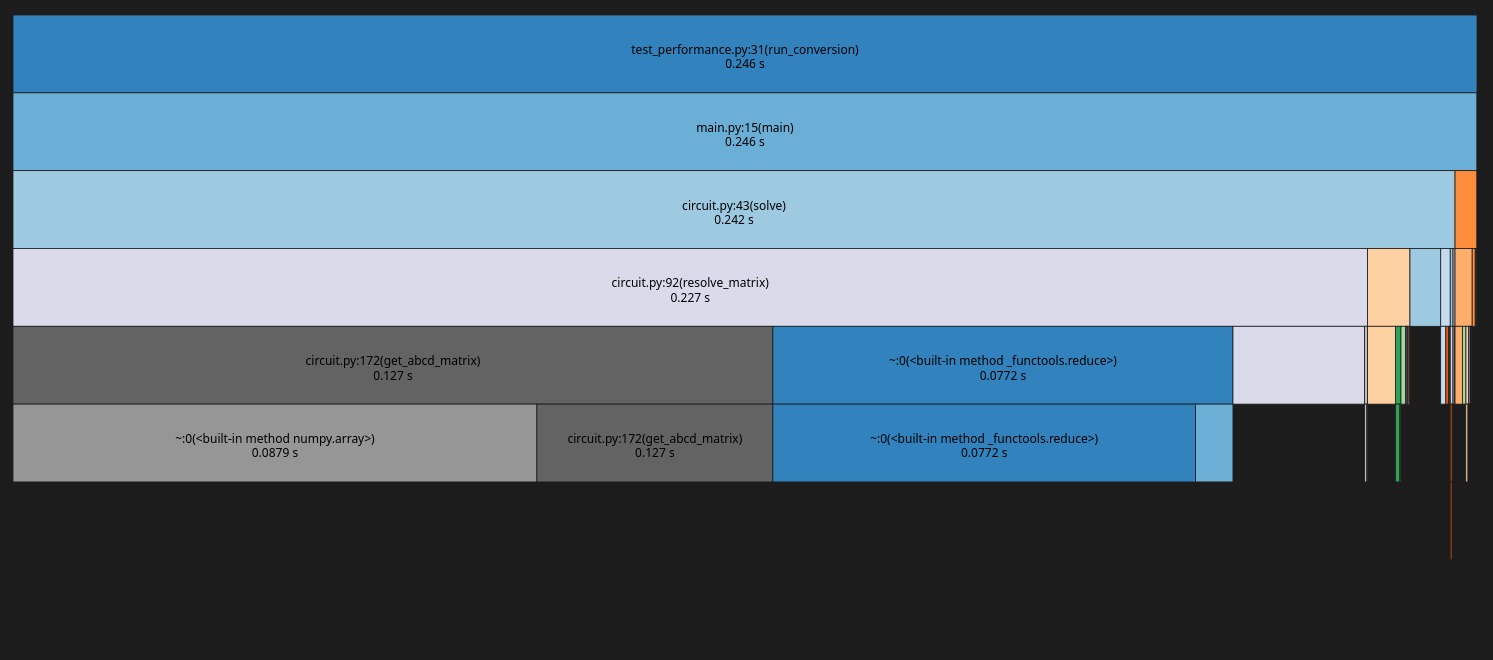
\includegraphics[width=\linewidth]{Images/Ext_e_Ladder_400.prof.png}
      \caption{Icicle graph of the cProfile run for the \texttt{Ext\_e\_Ladder\_400.net} test case.}
      \label{fig:ext_e_ladder_400}
\end{figure}


[2] \texttt{Ext\_mdB\_a\_Test\_Circuit\_1.prof}
\begin{figure}[ht]
      \centering
      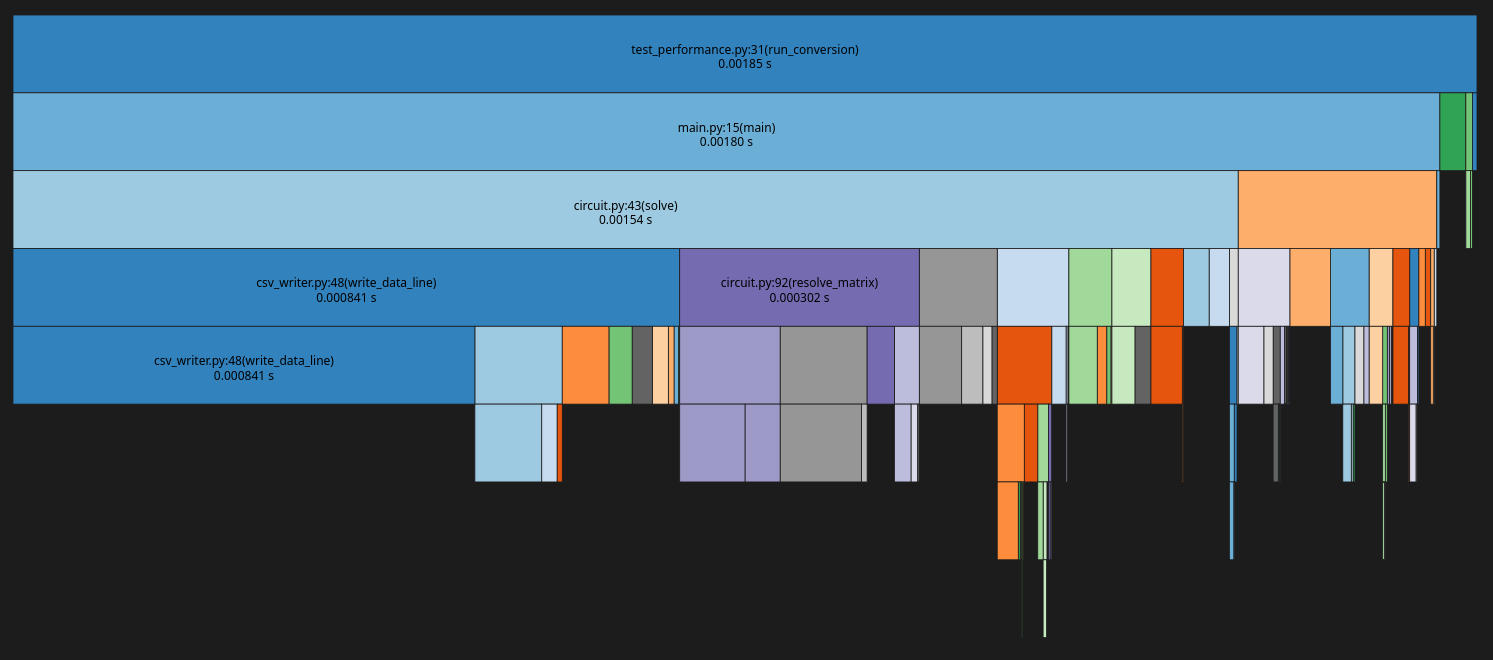
\includegraphics[width=\linewidth]{Images/Ext_mdB_a_Test_Circuit_1.prof.png}
      \caption{Icicle graph of the cProfile run for the \texttt{Ext\_mdB\_a\_Test\_Circuit\_1.net} test case.}
      \label{fig:ext_mdb_a_test_circuit_1}
\end{figure}

[3] \texttt{Record of Testing}
\begin{figure}[ht]
      \centering
      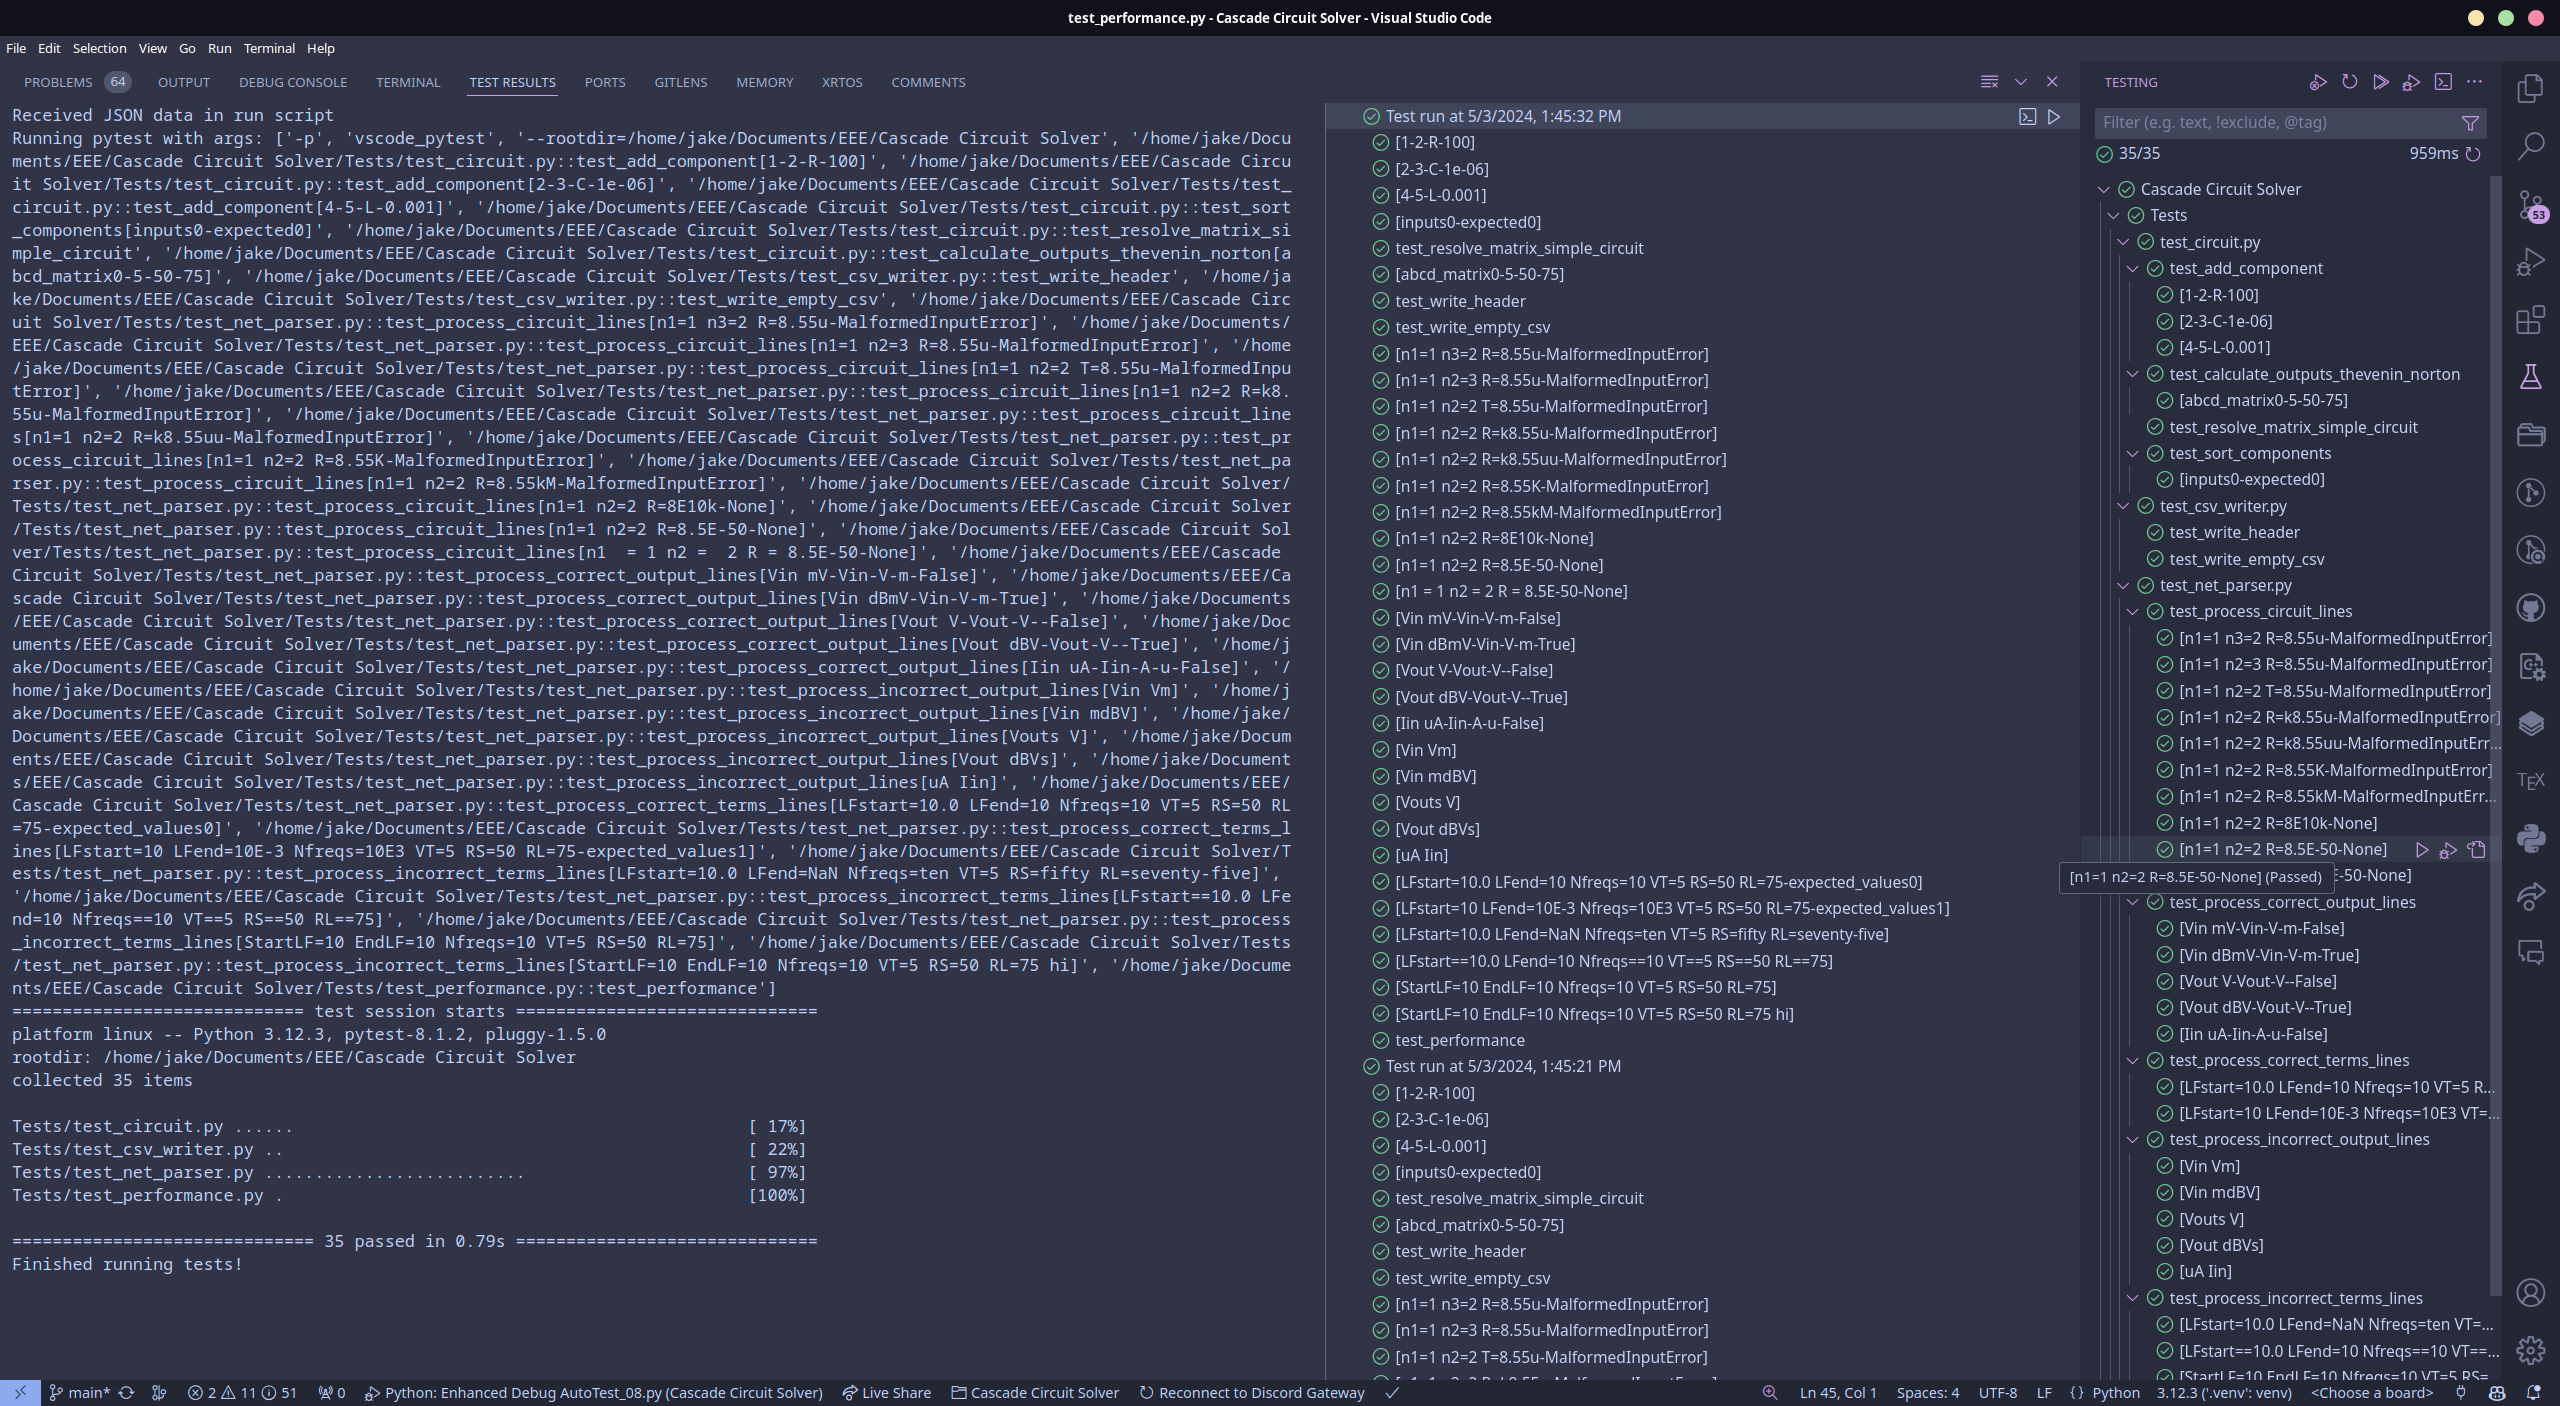
\includegraphics[width=\linewidth]{Images/Record of Testing.png}
      \caption{Screenshot from VSCode testing window, showing all tests passing.}
      \label{fig:record_of_testing}
\end{figure}

\end{document}